This section presents our measurement methodology and result on file system performance.

\subsection{Size of File Cache}

\subsubsection{Methodology}
File cache is adopted by the OS to improve the file access performance on disk. To measure the file cache size in our system, we generate files of different sizes and measure the average sequence read time of a block. The expectation is when the read file is small, the whole file could be cached in memory so the reading time would be as short as memory access; but when the file is large, the file cache is not enough to cache the whole file, so some read would cause cache miss and thus
leads to disk access, which is much longer than memory access. Based on this, our methodology determines the file cache size by observing on which file size, the access time increases largely.

More specifically, we created files of sizes from 128MB to 8GB increased by a step of 128MB. We choose the upper bound of file size since the total physical memory of the tested machine is 8GB. To bypass the cache in the C library, we use the \textbf{open()} system call directly instead of using the \textbf{fopen()} function call in C library. To Warm up the cache and to avoid outliers, each file is read for 11 times and the average of last 10 times is took as the result.

\subsubsection{Estimation and Results}
\label {File_cache_size_section}
Since the tested machine's total physical memory is 8GB, the linux kernel caches files very aggressive, and the tested system is Ubuntu, which usually takes less than 1GB memory, we estimate the file cache size would be between 7GB to 8GB.

%For access time, we estimate the per-block reading time of small files would be as same as a memory page copy. As \textbf{Section \ref{Memory_bandwidth_result_section}} shows, the memory read bandwidth is about 9356MB/s, so reading a 4K page would take 4KB/9356MB/s, namely \textbf{0.43us}. In contrast, the per-block reading time of large files would cause a disk access, and since the tested disk's data transfer rate is 300MB/s, we estimate the reading time of a 4K block would be 4KB/300MB/s, namely \textbf{13us}.

\begin{figure}[ht]
    \centering
    \frame{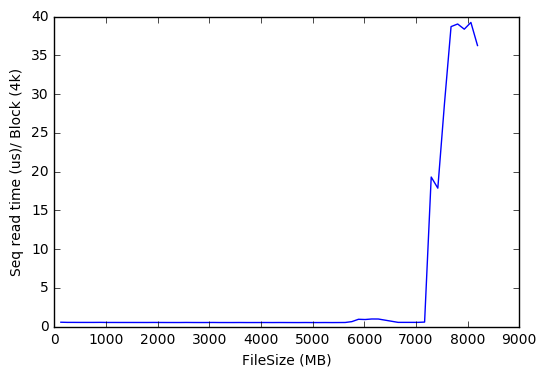
\includegraphics[width = .9\textwidth]{pictures/filecachesize.png}}
    \caption{Reading time of different sized files}
    \label{file_cache_size}
\end{figure}

\textbf{Figure \ref{file_cache_size}} shows how the measured read time varies against different file sizes. We can see that when the file size increases to 7296MB, the reading time increases largely, from 0.5us to 38us. So the file cache size should be about 7296MB (7.1GB), which is in the range we estimated.

\subsection{File Read Time}
\label {File_read_time_section}
\subsubsection{Methodology}
To measure the file read time without file cache, we use the \textbf{open()} system call with the flag \textbf{O_DIRECT}, which indicates reading directly from disk instead of cache. For sequential read time, we use \textbf{read()} to read a 4K block each time and accumulate the total time of reading from offset 0 to the file end. For random read time, we use \textbf{(rand()\%blocknum)*blocksize} to generate read offset and do the sampled read 1000 times for each file. We generate files of sizes from 4MB to 1GB as reading workload. And both the sequential read and random read test are conducted for 10 times and the average read time is calculated as the result

\subsubsection{Estimation and Results}
We estimate the sequential read time would only be determined by the disk data transfer rate, without seek time and rotation latency. So the sequential read time of different sized file would be the same. And since the max data transfer rate is 300Mbps (37.5MB/s), we estimate the sequential read time per block would be:

$$\frac{4KB}{37.5*1000KB/s} = 107us.$$

For the random read time, we take into account seek time and rotation latency. As the rotation speed is 7200RPM, the average rotation latency should be:

$$ \frac{\frac{60s}{7200}}{2} = 4.2ms.$$

And since the usual seek time of a hard disk is about 9ms, the random read time per block should be:
$$ 107us + 4.2ms + 9ms = 13.3ms. $$

And we estimate the random read time will increase as the file size increase, because large files may locates in many cylinders, which requires many head moving while be random read, while small files can be stored in a single cylinder, which requires no head moving.

\begin{figure}[ht]
    \centering
    \frame{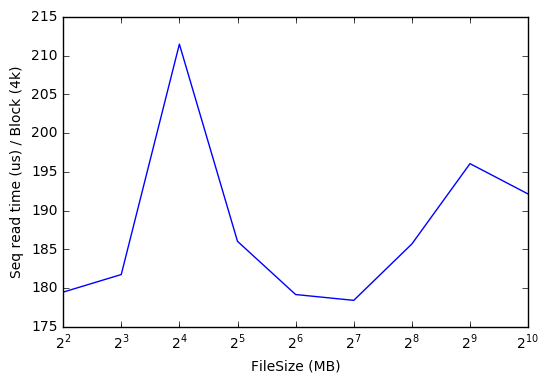
\includegraphics[width = .9\textwidth]{pictures/seqread.png}}
    \caption{Sequential read time per block (4KB)}
    \label{seq_read_time}
\end{figure}

\textbf{Figure \ref{seq_read_time}} shows sequential read time of different file sizes. The total average per-block read time is \textbf{187.8us}, which is a little longer than we estimated (107us). In addition, the read time varies when the file size increase. We speculate the reason is that a file is not totally stored in sequential disk sectors. The data blocks may be on different cylinders, especially for large files. So seeking time and rotation latency are also necessary for
sequential read. And since sequentially reading different-sized files need different times of seeking and rotation, the per-block read time varies. For large files, although more seeking and rotation may be required, but the large block number can also amortize the latency; therefore, a large file may have a shorter read time than a small file, as \textbf{Figure \ref{req_read_time}} shows.


\begin{figure}[ht]
    \centering
    \frame{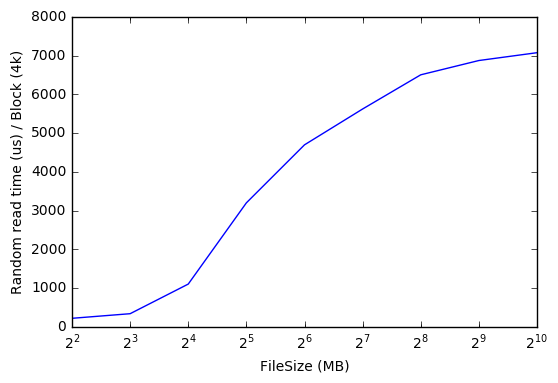
\includegraphics[width = .9\textwidth]{pictures/randread.png}}
    \caption{Random read time per block (4KB)}
    \label{rand_read_time}
\end{figure}

\textbf{Figure \ref{rand_read_time}} shows sequential read time of different file sizes. The average per-block read time increases as the file size increases, as we expected. As aforementioned, the reason is that large files span more sectors and cylinders than small files, so more seeking and rotation is needed for reading. And for small files (4MB to 16MB), increasing of file sizes only causes small increasing of read time, compared to that of large files (16MB to 512MB).
The reason is that file size increasing of small files only leads to more sectors while file size increasing of large files can cause more cylinders.

\subsection{Remote File Read Time}

\subsubsection{Methodology}
To test the read time of remote files, we set up a NFS sever on a different machine, as described in \textbf{Network}, and mount it on our main testing machine. The key challenge is to bypass both the server side and client side file cache. One possible way to address it is use \textbf{O_DIRECT} flag when call open(). However, that flag only take effect when the linux kernel support it, and unfortunately our testing system kernel doesn't support that. As a result,
we adopts another way: free the file cache before conducting test. That is implemented by calling:

\begin{lstlisting}
sudo sh -c 'echo 3>/proc/sys/vm/drop_caches'
\end{lstlisting}

And to avoid NFS transfers more than one block when a data block is read, we set the both read size and write size to 4KB:

\begin{lstlisting}
sudo mount dyn54:/export /mnt -o rsize=4096,wsize=4096
\end{lstlisting}


\subsubsection{Estimation and Results}
We estimate the network penalty with the round trip time and network bandwidth we have measured. \textbf{Section Network} shows that the measured round trip time is 0.338ms (338us) and the peak network bandwidth is 112MB/s, so the network penalty for a block should be:

$$\frac{4KB}{112*1000KB/s} + 338us = 373.7us$$

\begin{figure}[ht]
    \centering
    \frame{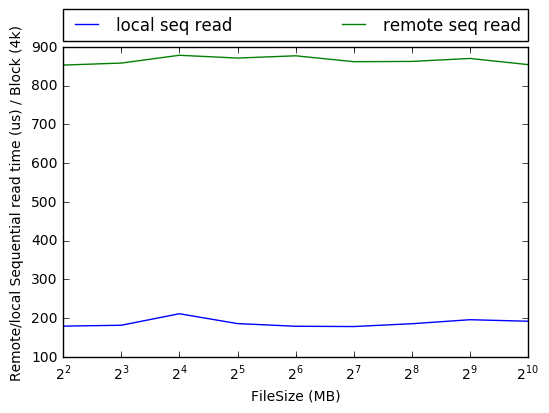
\includegraphics[width = .9\textwidth]{pictures/rseqread.png}}
    \caption{Remote/Local sequential read time per block (4KB)}
    \label{rseq_read_time}
\end{figure}

\textbf{Figure \ref{rseq_read_time}} shows both the remote and local sequential read time of different file sizes. The average per-block read time are 865.3us and 187.8us correspondingly. So the average network penaly is:

$$865.3us - 187.3us = 678us.$$

Compared with our estimated network penalty, the measured one is in the same order of magnitude but almost twice bigger. We speculate the reason is that the NFS implementation introduces additional overhead on read time.

\begin{figure}[ht]
    \centering
    \frame{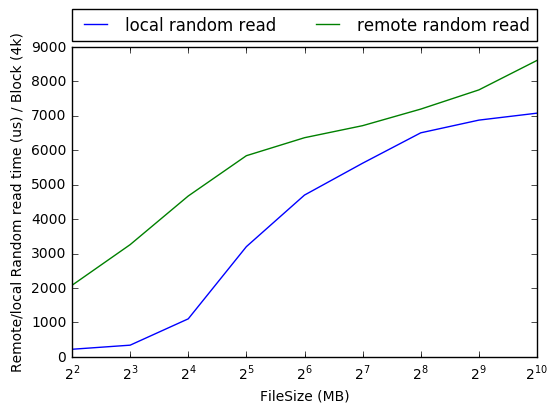
\includegraphics[width = .9\textwidth]{pictures/rrandread.png}}
    \caption{Remote/Local random read time per block (4KB)}
    \label{rrand_read_time}
\end{figure}

\textbf{Figure \ref{rseq_read_time}} shows both the remote and local random read time of different file sizes. The average per-block read time are 4365.2us and 3961.7us correspondingly. So the average network penaly is:

$$5832.3us - 3961.7us = 1870.5us.$$

This penalty is much bigger to the sequential reading one. We speculate the reason is that the remote disk needs more seeking time for random read. The remote disk is 160GB with 8MB cache while local disk is 750GB with 32MB cache. Since the capacity difference, one cylinder of the remote disk should have less sector than the local disk. So the same sized file on the remote disk would span more cylinder than on the local disk, which leads to more seeking time.

\subsection{Contention}
\subsubsection{Methodology}
To measure the contention effect of different process reading different files on the same disk, we generate \textbf{10} different files with the same size of \textbf{128MB} and create \textbf{1} to \textbf{10} processes to do the reading test. We uses the \textbf{open()} call with \textbf{O_DIRECT} to bypass the file cache, same as \textbf{Section \ref{File_read_time_section}}. To calculate the time of reading a block, we write test program to sequentially read the file once a block from the beginning to the end and calculate the average time as the result. We repeat the each test for 10 times to eliminate outerliers.

\subsubsection{Estimation and Results}
Since different processes share the same disk bandwidth when they read the same disk simultaneously, we estimate the reading time increases by times of the process number. As we measured before, the per-block read time of one process is 188us, we estimate contented read time would be:
$$process number * 188us$$

\begin{figure}[ht]
    \centering
    \frame{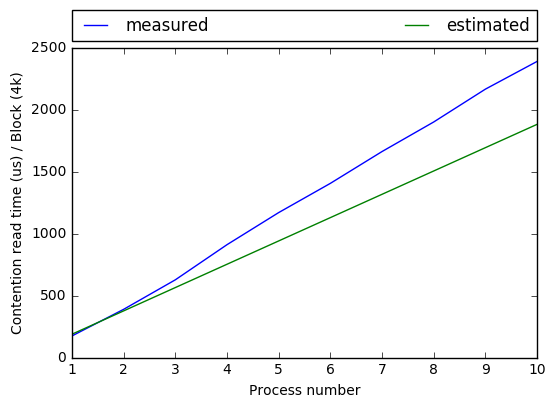
\includegraphics[width = .9\textwidth]{pictures/contention.png}}
    \caption{Remote/Local random read time per block (4KB)}
    \label{contention_read_time}
\end{figure}

\textbf{Figure \ref{contention_read_time}} show the per-block read time with contention of different process number. We can see that the measured read time increase linearly almost as the line:
$$ read time = 174 + process * 240 (us)$$
The measured read time is quite close to our estimation but a little bit higer. That is reasonable since we have not taken into account the process switch overhead.
